\section{Teoría de Conjuntos}

\subsection{Conjuntos y Elementos. Subconjuntos}


	Un \emph{conjunto} puede ser visto como un conjunto bien definido de objetos, llamados \emph{elementos} o \emph{miembros} de tal conjunto. 
	
	Usualmente, usaremos letras mayúsculas para denotar conjunto, y minúsculas para dlos elementos. 



	La pertenencia en un conjunto se denota de la siguiente manera:
	\begin{center}
		\emph{$a \in S$ denota que $a$ pertenece al conjunto $S.$} 
		
		\emph{$a,b \in S$ denota que tanto $a$ como $b$ pertenecen al conjunto $S.$}
	\end{center}
	
	El símbolo $\in$ significa \texttt{``es elemento de''.}  Por el contrario, $\notin$ significa \texttt{``no es elemento de''.}


\subsection{Especificación de Conjuntos}


	Básicamente, existen dos maneras de especificar un conjunto en particular.  Por un lado, si es posible, enlistar todos los miembros.  Por otro lado, caracterizando los elementos en el conjunto.



	En cualquier caso, para declarar un conjunto se utilizan llaves:
	$$
	A=\set{\cdots}
	$$



	Por ejemplo, el conjunto 
	$$
	A=\set{1,3,5,6,9}
	$$
	tambi\'en se puede especificar como
	$$
	A=\set{x\in \N \mid x<10, 2\nmid x }
	$$



	Un conjunto no depende del modo en que sus elementos se muestren.  Este permanece igual si sus elementos se repiten o se reacomodan.




	\begin{ejemplo}
		\begin{align*}
			\set{x\in\R | x^{2}-3x+2=0} & =\set{1,2} \\
			&=\set{1,2,2,1}
		\end{align*}
		
	\end{ejemplo}
	


\subsection{Subconjuntos}


	Supongamos que cada elemento en un conjunto $A$ es tambi\'en elemento del conjunto $B,$ es decir,
	$$
	x\in A \onlyif x\in B.
	$$



	En ese caso, decimos que $A$ es subconjunto de $B.$  Tambi\'en podemos decir que $A$ está contenido en $B$ o que $B$ contiene a $A$.



	Esta relación se escribe como
	$$
	A \subset B 
	$$ o en ocasiones como
	$B\supset A.$  Por el contrario, si es necesario indicar que $A$ \emph{no} es  subconjunto de $B,$ escribimos $A \not\subset B.$



	Diremos que dos conjuntos son iguales si poseen los mismos elementos, es decir, 
	$$
	x \in A \iff x \in B.
	$$



	De manera equivalente 
	\begin{center}
		$A=B$ si y solo si $A \subset B$ y $B \subset A.$
	\end{center}
	



	\begin{ejemplo}
		\label{lip:exmp:1.2}
		Determine la relación entre los siguientes conjuntos
		\begin{center}
			$$A=\set{1,3,4,7,8,9}, \, 
			B=\set{1,2,3,4,5}, \,
			C=\set{1,3}.$$
		\end{center}
		
	\end{ejemplo}
	



	\begin{ejemplo}
		Demuestre que 
		\begin{enumerate}
			\item $A\not\subset B$ si y solo $\exists x\in A: x\notin B.$
			\item $A \subset A.$
			\item $A\subset B, B\subset C \onlyif  A\subset C.$
		\end{enumerate}
		
	\end{ejemplo}
	


\subsection{Símbolos especiales}

 Algunos conjuntos num\'ericos tienen una notación especial
	\begin{itemize}
		\item $\N:$ números naturales (enteros positivos); 
		\item $\Z:$ números enteros; 
		\item $\Q:$ números racionales; 
		\item $\R:$ números reales; 
		\item $\mathbb{C}:$ números complejos.
	\end{itemize}
	
	



	Observe que
	$$
	\N \subset \Z \subset \Q \subset \R \subset \mathbb{C},
	$$ pero en ningún caso los conjuntos son iguales. 


\subsection{Conjunto Universal y Conjunto Vacío}


	Todos los conjuntos bajo investigación en una apliación de teoría de conjuntos se supone que pertenecen a un conjunto fijo más grande llamado \emph{conjunto universo} $\uset,$ al menos que se indique otro caso.



	Dado un conjunto universal $\uset$ y una propiedad $P,$ es posible que no existan elemento de $\uset$ con la propiedad $P.$ 



	Por ejemplo, el siguiente conjunto no tiene elementos
	$$
	S=\set{x\in \Z \mid x^{2}=3}.
	$$



	A tal conjunto sin elementos $\set{}$ se le conoce como conjunto vacío y se denota como $\emptyset.$



	\begin{observacion}
		\emph{Sólo existe un conjunto vacío}.  El conjunto vacío es subconjunto de cualquier otro conjunto.
	\end{observacion}
	


\subsection{Conjuntos disjuntos}


	Dos conjuntos $A$ y $B$ son \emph{disjuntos} si no tienen elementos en común. 



	\begin{ejemplo}
		Considere $$
		A=\set{1,2}, \; B=\set{4,5,6}, \; C=\set{5,6,7,8}.
		$$
		Determine que pares de conjuntos son disjuntos. 
	\end{ejemplo}
	


\subsection{Diagramas de Venn}


	Un diagrama de Venn es una representación gráfica de conjuntos en el que cada conjunto está representado por áreas encerradas en el plano.



	El conjunto universo $\uset$ es representado por el interior de un rectángulo, y cualquier otro conjunto esta representado por discos que viven dentro del rectángulo.



	\begin{figure}
		\centering
		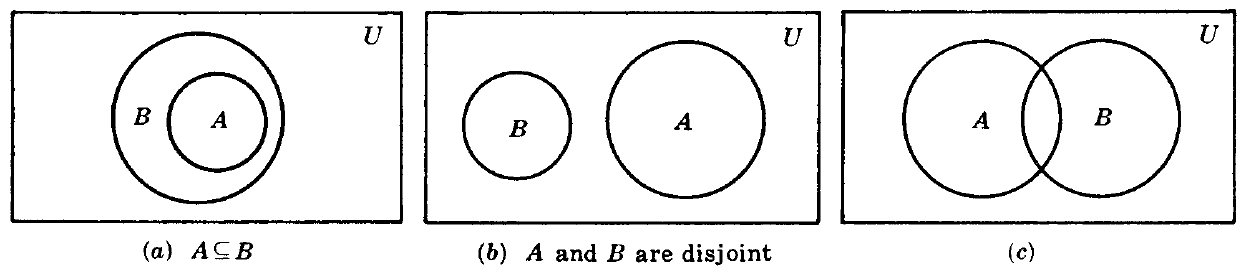
\includegraphics[width=11cm,keepaspectratio=true]{./md/venn01.png}
		% venn01.png: 0x0 pixel, 300dpi, 0.00x0.00 cm, bb=
		\caption{Representaciones con Diagramas de Venn}
		\label{fig:0101}
	\end{figure}
	


\subsection{Operaciones con Conjuntos}


	En esta sección introduciremos la unión, la intersección y el complemento de conjuntos.


\subsection{Unión e Intersección}


	La unión de dos conjuntos $A$ y $B$ es el conjunto de todos los elementos que pertenecen a $A$ o a $B,$  es decir
	$$
	A \cup B = \set{x \mid x\in A \vee x\in B}.
	$$



	La intersección de dos conjuntos $A$ y $B$ es el conjunto de todos los elementos que pertenecen a $A$ y a $B,$  es decir
	$$
	A \cap B = \set{x \mid x\in A \wed x\in B}.
	$$



	\begin{figure}
		\centering
		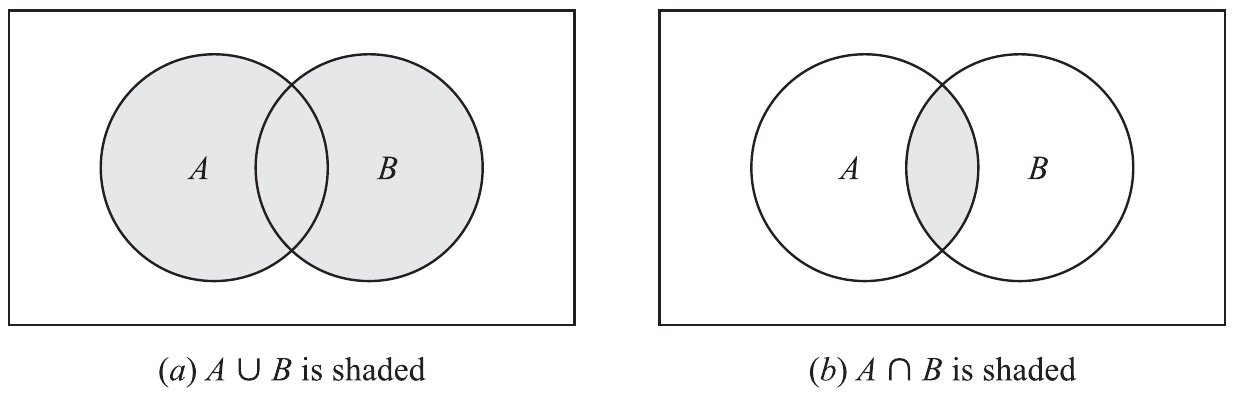
\includegraphics[width=10cm,keepaspectratio=true]{./md/venn_union_interseccion.png}
		% venn_union_interseccion.png: 0x0 pixel, 300dpi, 0.00x0.00 cm, bb=
		\caption{Unión e Intersección}
		\label{fig:0103}
	\end{figure}
	








